\section{Probability Density Estimation}
% -----------------------------------------------------------------------------
This chapter introduces the concept of a probability density and illustrates both \emph{non-parametric} ($\rightarrow$ section \ref{sec:KDE})  and \emph{parametric} ($\rightarrow$ section \ref{sec:ParametricDensityEstimation}) approaches to estimate a density function given limited amounts of data. Good estimators can often be constructed using the \emph{Maximum Likelihood} principle, which is illustrated in section \ref{sec:ML}.  

% \subsection{Probability Densities and Problem Statement}
\paragraph{Probabilities}
\[ \begin{array}{ll}
	\text{discrete random variable:} & X \\\\
	\text{values:} & x \in X = \big\{ x_1, x_2, \ldots, x_k \big\} \\\\
	P(x): & X \rightarrow \mathbb{R} \\\\
	\text{positivity and normalization:} & 0 \leq P(x) \leq 1 
		\text{ and } \sum\limits_{i} P(x_i) = 1
\end{array} \]

\paragraph{Probability Density}
\[ \begin{array}{ll}
	\text{continous random variable:} & X \\\\
	\text{values:} & x \in \mathbb{R} \text{ (can be generalised to } \mathbb{R}^n, P(\vec{x}) \text{)} \\\\
	\text{probability density:} 
		& P(x): \mathbb{R} \rightarrow \mathbb{R}_0^+ \\
	& \leadsto \text{ non-negative function}\\
	& \leadsto \text{ normalized to }
		\int_{\mathrm{support(x)}} d x P(x) = 1\\
	& \leadsto  P(x) \text{ can be larger than } 1 \text{ for some } x \\\\
	\text{probability:} & \underbrace{ P(x)^{(\text{vol.})} 
						= \int_{\text{vol.}}dxP(x)}_{
				\text{\underline{p}robability 
					\underline{d}ensity
					\underline{f}unction (pdf)}} \\\\
	\text{probability density:} & \frac{\text{probability}}{\text{volume}}
\end{array} \] 

\paragraph{Density Estimation}\mbox{}\\\\
Given observations $\vec{x}^{(\alpha)}, \alpha = 1, \ldots, p$ drawn
(iid) from a (generally unknown) distribution, \emph{inductive
  learning} can be applied to get good estimates for both prior
densities $P(x)$ and conditional densities $P(y|x)$.
\[ \text{''good'' estimate/model } \widehat{P}(\vec{x})
\left \{ \begin{array}{ll}
	\text{non-parametric methods (e.g. histograms)} \\\\
	\text{parametric methods: } \widehat{P}(\vec{x};\vec{w})\\
	\leadsto \text{ estimate a ''good'' parameter vector } \vec{w}
\end{array} \right. \]


% -----------------------------------------------------------------------------
\subsection{Kernel Density Estimation} \label{sec:KDE}
\begin{center}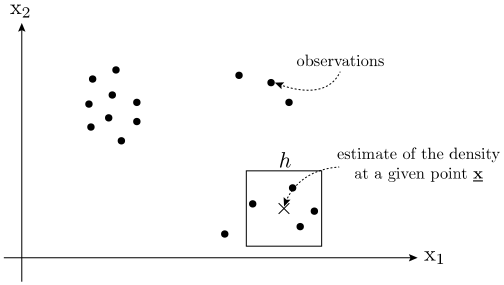
\includegraphics[height=5cm]{section1_fig1}
\end{center}

\paragraph{Histogram:} count the number of data points in a volume of a given size $V$ centered on $\vec{x}$. For $u_j=\vec{x}_j - \vec{x}^{(\alpha)}_j $
\begin{equation}
	\begin{array}{ll}
		V = h^n & \text{volume} \\\\
		H(\vec{u}) = \left \{ \begin{array}{ll}
			1, & |u_j| < \frac{1}{2}, \forall j \in 1, \ldots, n \\\\
			0, & \text{else}
			\end{array} \right.
			& \substack{ \text{histogram ''kernel''} \\
				\text{(here: equals to } 1 \\
				\text{if } \vec{u} \text{ is located within}\\
				\text{the unit cube)}}
	\end{array}
\end{equation}

\paragraph{Density estimate} (''gliding histogram'')
\begin{equation}
	\widehat{P}(\vec{x}) = \underbrace{ \frac{1}{h^n} }_{
					\substack{ \text{normalization} \\
						\text{(''density''!)}}}
				\cdot \underbrace{ \frac{1}{p} 
				\overbrace{ \sum\limits_{\alpha = 1}^p
				H \bigg( \frac{\vec{x} - \vec{x}^{(\alpha)}}{
						h} \bigg) }^{
					\substack{\text{number of data points}\\
						\text{within volume } V 
						\text{ around } \vec{x}}} }_{
					\text{fraction of data points}}
\end{equation}
\emph{Problem:} Histogram kernel leads to discontinous pdf estimates $\leadsto$ use other kernel than the 'box' to get smooth pdf-estimates. 
\begin{itemize}
	\itl weighted sum of data points
	\itl e.g. through a Gaussian kernel \\
		\begin{equation}
			H(\vec{u}) = \frac{1}{(2\pi)^{\frac{n}{2}}} 
				\exp \bigg( -\frac{\vec{u}^2}{2} \bigg)
		\end{equation}
\end{itemize}
\begin{center}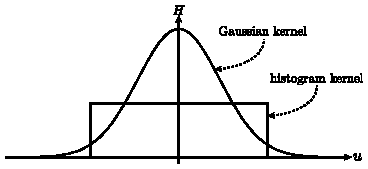
\includegraphics[height=5cm]{section1_fig2}
\end{center}
Density estimate:
\begin{equation}
	\begin{array}{ll}
	\widehat{P}(\vec{x}) 
	& = \frac{1}{h^n} \cdot \frac{1}{p} \sum\limits_{\alpha = 1}^p
		H \Big( \frac{\vec{x} - \vec{x}^{(\alpha)}}{h} \Big) \\\\
	& = \frac{1}{p} \sum\limits_{\alpha = 1}^p \frac{1}{
				\big(2\pi h^2\big)^{\frac{n}{2}}}
			\exp \bigg\{ -\frac{\big(\vec{x} - \vec{x}^{(\alpha)}
						\big)^2}{2h^2} \bigg\}
	\end{array}
\end{equation}
$h$: hyperparameter $\leadsto$ determines smoothness
\\
\begin{figure}[h]
  \centering
  \includegraphics[width=\textwidth]{densExamples.pdf}
  \caption{Impact of kernel-width on density estimate.}
  \label{fig:kernelWidth}
\end{figure}
\\
optimal choice of $h$? $\rightarrow$ see section \ref{sec:ERMDE}


% -----------------------------------------------------------------------------
\subsection{Parametric Density Estimation}
\label{sec:ParametricDensityEstimation}
Given a set of observations $\big\{ \vec{x}^{(\alpha)} \big\}, \alpha = 1, \ldots, p$, we assume the data has been 
produced by a specific \emph{generative model}, e.g.\ a
parameterized family of pdfs: $\widehat{P}(\vec{x};\vec{w})$ 
\[ \begin{array}{lcl}
	\fbox{$ \substack{ \text{generative model} \\ \text{of a data source} 
		} $}
	& \longrightarrow & \fbox{$ \text{observations} $} \\\\
	\substack{ \text{description of the} \\ \text{generation process} }
\end{array} \]
\textbf{Comment:}
\[ \begin{array}{lll}
	\text{MI 2:} & \text{models } \widehat{P}(\vec{x};\vec{w}) \text{ for
		unconditional densities } P(\vec{x}) 
		& \leftarrow \text{ unsupervised learning} \\\\
	\text{MI I:} & \text{models } \widehat{P}(y|\vec{x};\vec{w}) \text{ for
		conditional densities } P(y|\vec{x})
		& \leftarrow \text{ supervised learning}
\end{array} \]
\subsubsection{Model Selection and Cost function}
Select the model which is most similar to the true density! 
\\\\
Kullback-Leibler-Divergence
\begin{equation}
	\dkl = \int d \vec{x} P(\vec{x}) \ln 
		\frac{P(\vec{x})}{\widehat{P}(\vec{x};\vec{w})}
\end{equation}
\begin{itemize}
	\itr distance measure between probability distributions
\end{itemize}
$\dkl \geq 0$ and $\dkl = 0$ iff $\widehat{P}(\vec{x};\vec{w}) = P(\vec{x})$
\\\\
Criterion for model selection:
\begin{equation}
	\dkl \eqexcl \min_{(\vec{w})}
\end{equation}
\begin{equation}
	\begin{array}{lll}
	\vec{w}^* 
	& = \argmin_{\vec{w}} \Big\{ \int d \vec{x} P(\vec{x}) \ln P(\vec{x})
		- \int d \vec{x} P(\vec{x}) \ln \widehat{P}(\vec{x};\vec{w})
		\Big\} \\\\
	& = \argmin_{\vec{w}} \Big\{ \underbrace{ -\int d \vec{x} P(\vec{x}) 
		\ln \widehat{P}(\vec{x};\vec{w}) }_{ E_{[\vec{w}]}^G } \Big\} 
		& \text{{\small ''cross entropy''}}
	\end{array}
\end{equation}
\begin{equation}
	E^G \eqexcl \min_{(\vec{w})}
\end{equation}
problem: $P(\vec{x})$ is unknown.
\\\\
\subsubsection{Principle of empirical risk minimization (ERM)}
\label{sec:ERMDE}
\[ \begin{array}{ccc}
	\fbox{$ \substack{ \text{mathematical} \\ \text{expectation } E^G} $}
	& \longrightarrow & \fbox{$ \substack{ \text{empirical} \\ 
		\text{average } E^T} $}
	\\\\
	\text{{\small ''generalization cost''}} && 
	\text{{\small ''training cost''}}
\end{array} \]
cost function:
\begin{equation}
	E^T = -\frac{1}{p} \sum\limits_{\alpha = 1}^p \ln 
		\widehat{P}\big( \vec{x}^{(\alpha)};\vec{w} \big) 
\end{equation}
but when is this a reasonable procedure? $\leadsto$ statistical learning theory
\\
{\it (cf. MI I, section 2.1)}
\\\\
criterion for model selection:
\begin{equation}
	\fbox{$ E^T = -\frac{1}{p} \sum\limits_{\alpha = 1}^p \ln 
		\widehat{P}\big( (\vec{x}^{(\alpha)};\vec{w} \big)
		\eqexcl \min_{(\vec{w})} $}
\end{equation}

\paragraph{Optimization}
\begin{equation}
	\underbrace{ E_{[\vec{w}]}^T }_{ \substack{\text{total} \\ \text{cost}}}
		= \frac{1}{p} \sum\limits_{\alpha = 1}^p 
		\underbrace{ e_{[\vec{w}]}^{(\alpha)} }_{
			\substack{ \text{individual} \\ \text{cost} }}
\end{equation}
standard gradient-descent procedures {\it (cf. MI I, sections 1.3.4 and 1.4.1-3)}
\begin{equation}
	\left.  \begin{array}{ll}
	\text{''batch''-learning:} 
		& \Delta \vec{w} = -\eta \frac{\partial E^T}{\partial \vec{w}}
		\\\\
	\text{''on-line''-learning:}
		& \Delta \vec{w} = -\eta \frac{\partial e^{(\alpha)}}{\partial
			\vec{w}}
	\end{array} \right \} 
	\substack{ \text{examples for} \\ 
			\text{gradient-based} \\
			\text{methods}}
\end{equation}

\paragraph{Validation}\mbox{}
\\\\
\emph{Motivation:} $E_{[\vec{w}]}^T \eqexcl \min$ instead of $E_{[\vec{w}]}^G \eqexcl \min$ may lead to overfitting.
\begin{center}\includegraphics[height=5cm]{section1_fig3}
\end{center}
$E^T$ small but $E^G$ large may indicate overfitting
\\\\
\emph{Testset method:}
\[ \text{observations} \left\{ \begin{array}{ll}
	\text{training data} & \big\{ \vec{x}^{(\alpha)} \big\}, \alpha = 1, 
		\ldots, p \\\\
	\text{test data} & \big\{ \vec{x}^{(\beta)} \big\}, \beta = 1, 
		\ldots, q
\end{array} \right. \]
\begin{equation}
	\widehat{E}^G = \frac{1}{q} \sum\limits_{\beta = 1}^q e^{(\beta)}
		\leftarrow \text{ estimate of } E^G
\end{equation}
\begin{center}\includegraphics[height=5cm]{section1_fig4}
\end{center}
\begin{itemize}
	\itR $E_{(I)}^T > E_{(II)}^T$ \underline{but} $E_{(I)}^G << E_{(II)}^G$
\end{itemize}
alternative to the ``test-set-method'': n-fold cross-validation {\it
  (cf. MI I, section 1.3.7)}
\\\\
\textbf{Comment:} Validation methods can also be used to estimate
hyperparameters for non-parametric methods (i.e. kernel density
estimate).

% -----------------------------------------------------------------------------

% -----------------------------------------------------------------------------


\subsubsection{The Principle of Maximum Likelihood} \label{sec:ML}
generative model
\begin{equation}
        \begin{array}{lr}
        \widehat{P}(\vec{x};\vec{w}) 
        & \substack{ \text{probability density for the} \\
                   \text{generation of one data point} }
        \end{array}
\end{equation}
likelihood of the observations (iid assumption)
\begin{equation}
        \begin{array}{lr}
                \widehat{P}\big( \big\{ \vec{x}^{(\alpha)} \big\};\vec{w} \big)
                = \prod\limits_{\alpha = 1}^p \widehat{P}\big(\vec{x}^{(\alpha)}
                        ;\vec{w} \big)
                & \substack{    \text{probability density for the} \\
                                \text{generation of the whole} \\
                                \text{observed data set} }
        \end{array} 
\end{equation}
model selection via the maximum likelihood principle
\begin{equation}
        \widehat{P}\big(\big\{\vec{x}^{(\alpha)}\big\};\vec{w}\big)
                \eqexcl \max_{(\vec{w})}
\end{equation}
\emph{Idea:} pick the model under which the probability of observing the data is maximal\\\\
\emph{In practice:} minimization of the negative $\log$-likelihood
\begin{equation}
        \begin{array}{ll}
                p \cdot E_{[\vec{w}]}^T
                & = -\ln \widehat{P}\big(\big\{\vec{x}^{(\alpha)}\big\}
                        ;\vec{w}\big) \\\\
                & = -\sum\limits_{\alpha = 1}^p \ln \widehat{P}
                        \big( \vec{x}^{(\alpha)};\vec{w} \big) \\\\
                & \eqexcl \min
        \end{array}
\end{equation}
\begin{itemize}
        \itR fully equivalent to the minimization of the KL-divergence via ERM.
\end{itemize}

\paragraph{The multivariate Gaussian}
\vspace{-0.8cm}
\begin{alignat*}{2}
&\widehat{P}\left(\left\{ \vec{x}^{(\alpha)} \right\}; \vec{\boldsymbol \mu}, \vec{\Sigma} \right) &&= \left( \frac{1}{\sqrt{(2\pi)^N \det \vec{\Sigma}}} \right)^p \cdot \prod_{\alpha=1}^{p} \exp \left(-\frac{1}{2} \left(\vec{x}^{(\alpha)} - \vec{\boldsymbol \mu} \right)^T \vec{\Sigma}^{-1} \left(\vec{x}^{(\alpha)} - \vec{\boldsymbol \mu} \right) \right) \\[10pt]
&E^T\left( \vec{\boldsymbol \mu}, \vec{\Sigma} \right) &&= - \ln \widehat{P}\left(\left\{ \vec{x}^{(\alpha)} \right\}; \vec{\boldsymbol \mu}, \vec{\Sigma} \right) \\
& &&= \frac{p \cdot N}{2} \ln(2\pi) + \frac{p}{2} \ln(\det \vec{\Sigma}) + \frac{1}{2} \sum_{\alpha=1}^{p} \left(  \vec{x}^{(\alpha)} - \vec{\boldsymbol \mu} \right)^T \vec{\Sigma}^{-1} \left(  \vec{x}^{(\alpha)} - \vec{\boldsymbol \mu} \right)
\end{alignat*}
\\\vspace{0.2cm}
minimization of $E^T$ (necessary conditions):
\vspace{-0.1cm}
\begin{align*}
\frac{\partial E^T}{\partial \vec{\boldsymbol \mu}} = \vec{0} \quad &\Rightarrow \quad \vec{\boldsymbol \mu}^* = \frac{1}{p} \sum_{\alpha=1}^{p} \vec{x}^{(\alpha)}  &&\text{(empirical average)}\\
\frac{\partial E^T}{\partial \vec{\Sigma}} = \vec{0} \quad &\Rightarrow \quad \vec{\Sigma}^* = \frac{1}{p} \sum_{\alpha=1}^{p} (\vec{x}^{(\alpha)} - \vec{\boldsymbol \mu}^*) (\vec{x}^{(\alpha)} - \vec{\boldsymbol \mu}^*)^T &&\text{(empirical covariance matrix)}
\end{align*}

remark: $\vec{\boldsymbol \mu}^*$ is unbiased, but $\vec{\Sigma}^*$ is a biased estimator (cf. section: 6.1 Model fitting)
\newpage
\section{Mixture Models and the EM-Algorithm}
\subsection{Mixture Models}
\subsubsection{Motivation}
\begin{figure}[h]
    \centering
    \begin{subfigure}[b]{0.48\textwidth}
        \includegraphics[width=0.75\textwidth]{KMeans-Gaussian-data.png}
        \caption{K-Means Clustering}
    \end{subfigure}
    \begin{subfigure}[b]{0.48\textwidth}
        \includegraphics[width=0.75\textwidth]{EM-Gaussian-data.png}
        \caption{Mixture of Gaussians}
    \end{subfigure}
\end{figure}
\begin{figure}[h]
\centering
\includegraphics[width=7cm]{section6_fig1}
\caption{Component-based modeling of complex densities\citep{Bishop2006}}
\end{figure}

\paragraph{Data sources \& representation}\mbox{}\\
Data source $\rightarrow$ data $\vec{x} \in \mathbb{R}^N \sim P_{(\vec{x})}$\\
\begin{figure}[h]
  \centering
  \includegraphics[width=7cm]{section6_fig2}
  \label{fig:data_source}
\end{figure}
\vspace{-4mm}
$\Rightarrow$ Assumption: Data is generated by multiple sources / classes as represented by components in figure \ref{fig:data_source}

\paragraph{Model class}\mbox{}\\
$P_{(\vec{x} | q)}:$ components: probability density, that data point $\vec{x}$ was created by component $q$
\\\vspace{0.3cm}
$P_{(q)}:$ mixture parameters: probability, that component $q$ creates a data point
\begin{figure}[h]
	\centering
	\includegraphics[width=7cm]{section6_fig3}
\end{figure}
\begin{figure}[h]
	\centering
	\includegraphics[width=7cm]{section6_fig4}
\end{figure}

$\rightarrow$ deeper trees possible: hierarchical mixture-models \\\vspace{0.3cm}
$\rightarrow$ neural networks at the leaves: mixture of experts

\paragraph{Choice of basis functions}\mbox{}\\
\begin{align}
P_{(\vec{x})} &= \sum_{q=1}^{M} P_{(q)} P_{(\vec{x} | q)} \\
P_{(\vec{x} | q)} &= \mathcal{N}\left( \vec{x}; \vec{w}_q, \sigma_q^2 \right) = \frac{1}{(2\pi \sigma_q^2)^{N/2}} \exp \left\{ - \frac{(\vec{x} - \vec{w}_q)^2}{2\sigma_q^2} \right\} \\
&\leadsto \text{ (Gaussian mixture model)}
\end{align}\\\vspace{0.3cm}
parameters $P_{(q)}$, $\vec{w}_q$ and $\sigma_q$ must be determined for all components $q$ \\\vspace{0.3cm}
different basis functions are possible (problem specific)

\paragraph{Performance measure}
Probability, that the dataset $\left\{ \vec{x}^{(\alpha)} \right\}$ was generated by the model:
\begin{align}
P_{\left( \left\{ \vec{x}^{(\alpha)} \right\} \right)} = \prod_{\alpha=1}^{p} P_{(\vec{x}^{(\alpha)})} &= \prod_{\alpha=1}^{p} \left\{ \sum_{q=1}^{M} P_{(\vec{x}^{(\alpha)} | q)} P_{(q)} \right\} \\
&= \prod_{\alpha=1}^{p} \left\{ \sum_{q=1}^{M} \mathcal{N}\left( \vec{x}^{(\alpha)}; \vec{w}_q, \sigma_q^2 \right) P_{(q)} \right\}
\end{align}
Principle of maximum likelihood:
\begin{equation}
P_{\left( \left\{ \vec{x}^{(\alpha)} \right\} \right)} \eqexcl \max \quad \text{w.r.t. parameters}
\end{equation}
Minimization of negative log-likelihood instead:
\begin{equation}
E^T = - \ln P_{\left( \left\{ \vec{x}^{(\alpha)} \right\} \right)} = - \sum_{\alpha=1}^{p} \ln \sum_{q=1}^{M} P_{(\vec{x}^{(\alpha)} | q)} P_{(q)} \eqexcl \min \quad \text{w.r.t parameters}
\end{equation}

\paragraph{Relation to Soft-Clustering methods}
\small
Assumptions:
\begin{itemize}
	\item Gaussian mixture model with $M$ components
	\item same widths $\sigma_q^2 = \sigma^2 \coloneqq \underbrace{\frac{1}{\beta}}_{\text{given}}$ for all basis functions
	\item same mixture parameters $P_{(q)} = \frac{1}{M}$
\end{itemize}
\vspace{0.2cm}
Cost function: 
\begin{equation}
P_{(\vec{x}^{(\alpha)})} = \sum_{q=1}^{M} \mathcal{N}\left( \vec{x}^{(\alpha)}; \vec{w}_q, \sigma^2 \right) P_{(q)} = \frac{1}{M}\left(\frac{\beta}{2\pi}\right)^{N/2} \sum_{q=1}^{M} \exp \left\{ - \frac{\beta}{2} \left( \vec{x}^{(\alpha)} - \vec{w}_q \right)^2 \right\} 
\end{equation}
\vspace{-2mm}
\begin{align}
E^T = - \ln P_{\left( \left\{ \vec{x}^{(\alpha)} \right\} \right)} &= -\ln \prod_{\alpha=1}^{p} \left\{ \sum_{q=1}^{M} \mathcal{N}\left( \vec{x}^{(\alpha)}; \vec{w}_q, \sigma^2 \right) P_{(q)} \right\} 
\\&= - \sum_{\alpha=1}^{p} \ln \sum_{q=1}^{M} \exp \left\{ - \frac{\beta}{2} \left( \vec{x} - \vec{w}_q \right)^2 \right\} + \text{const}_{(\vec{w}_q)}
\end{align}
Assignment probabilities:\\\vspace{3mm}
$P_{(q | \vec{x})}$: posterior probability of component q having generated a given data point $\vec{x}$
\begin{equation}
P_{(q | \vec{x})} = \frac{P_{(\vec{x} | q)} P_{(q)}}{P_{(\vec{x})}} \qquad \text{(Bayes' theorem)}
\end{equation}
$\leadsto$ given the simplified Gaussian mixture model we obtain:
\begin{eqnarray}
P_{(q | \vec{x})} &=& \frac{\left( \frac{\beta}{2\pi} \right)^{N/2} \exp \left\{ - \frac{\beta}{2} \left( \vec{x} - \vec{w}_q \right)^2 \right\} \cdot \frac{1}{M}}{\left( \frac{\beta}{2\pi} \right)^{N/2} \frac{1}{M} \sum_{\gamma}^{} \exp \left\{ - \frac{\beta}{2} \left( \vec{x} - \vec{w}_{\gamma} \right)^2 \right\}} \\
&=& \frac{\exp \left\{ - \frac{\beta}{2} \left( \vec{x} - \vec{w}_q \right)^2 \right\}}{ \sum_{\gamma=1}^{M} \exp \left\{ - \frac{\beta}{2} \left( \vec{x} - \vec{w}_{\gamma} \right)^2 \right\}}
\end{eqnarray}
$\Rightarrow$ assignment probability for Soft-Clustering

\begin{equation}
E^T = - \sum_{\alpha=1}^{p} \ln \sum_{q=1}^{M} \exp \left\{ - \frac{\beta}{2} \left( \vec{x} - \vec{w}_q \right)^2 \right\} + \text{const}_{(\vec{w}_q)}
\end{equation}
Minimization of the cost function w.r.t. the weights:
\begin{align}
\frac{\partial E^T}{\partial \vec{w}_r} &= - \sum_{\alpha=1}^{p} \frac{\exp \left\{ - \frac{\beta}{2} \left( \vec{x} - \vec{w}_r \right)^2 \right\}}{\sum_{q=1}^{M} \exp \left\{ - \frac{\beta}{2} \left( \vec{x} - \vec{w}_q \right)^2 \right\}} \beta \left( \vec{x} - \vec{w}_r \right) \eqexcl 0 \\
\vec{w}_r &= \frac{\sum_{\alpha=1}^{p} P_{(r | \vec{x}^{(\alpha)})} \vec{x}^{(\alpha)}}{\sum_{\alpha=1}^{p} P_{(r | \vec{x}^{(\alpha)})}} \quad \leadsto \substack{\text{ center of mass condition}\\\text{for Soft-Clustering!}}
\end{align}
\begin{itemize}
	\item[\textcolor{black}{$\Rightarrow$}] Gaussian mixture model with components of equal size and strength is equivalent to Soft-Clustering
\end{itemize}
New interpretation of Soft-Clustering:
\begin{itemize}
	\item parameter estimation for a Gaussian mixture model with components of equal widths and strengths
	\item $\beta$ is given
	\item implicit assumption: every cluster contains the same number of data points
\end{itemize}
\vspace{0.5cm}
Mixture models can be viewed as an extension of Soft-Clustering methods:
\begin{itemize}
	\item clusters with different widths
	\item clusters with different number of data points
\end{itemize}
%-------------------------------------------------------------------------
\paragraph{Optimization for Gaussian mixtures}\mbox{}\\
\vspace{-0.3cm}
\small
Supporting equations:
\smaller
\begin{align*}
\frac{\partial}{\partial \vec{w}_q} P_{(\vec{x}^{(\alpha)} | q)} = \frac{\left( \vec{x} - \vec{w}_q \right)}{\sigma_q^2} P_{(\vec{x}^{(\alpha)} | q)} \qquad
\frac{\partial}{\partial \sigma_q} P_{(\vec{x}^{(\alpha)} | q)} = \left\{ -\frac{N}{\sigma_q} + \frac{\left( \vec{x} - \vec{w}_q \right)^2}{\sigma_q^3} \right\} P_{(\vec{x}^{(\alpha)} | q)}
\end{align*}
\small
Cost function:
$\quad
E^T = - \ln P_{\left\{ \vec{x}^{(\alpha)} \right\}} = - \sum_{\alpha=1}^{p} \ln \left( \sum_{q=1}^{M} P_{(\vec{x}^{(\alpha)} | q)} P_{(q)} \right) \eqexcl \min
$\\\vspace{0.2cm}
Minimization w.r.t. weights:
\begin{align*}
\frac{\partial E^T}{\partial \vec{w}_r} &= - \sum_{\alpha = 1}^{p} \frac{\frac{\left( \vec{x}^{(\alpha)} - \vec{w}_r \right)}{\sigma_r^2} \color{blue}{P_{(\vec{x}^{(\alpha)} | r)} P_{(r)}}}{\color{blue}{ \sum_{q=1}^{M} P_{(\vec{x}^{(\alpha)} | q)} P_{(q)}}} \\
&= \sum_{\alpha=1}^{p} \frac{\left( \vec{w}_r - \vec{x}^{(\alpha)} \right)}{\sigma_r^2} \color{blue}{P_{(r | \vec{x}^{(\alpha)})}} \color{black} \eqexcl 0
\end{align*}
\begin{equation*}
\boxed{\vec{w}_r = \frac{\sum_{\alpha=1}^{p} P_{(r | \vec{x}^{(\alpha)})} \vec{x}^{(\alpha)}}{\sum_{\alpha = 1}^{p} P_{(r | \vec{x}^{(\alpha)})}}}
\end{equation*}
$\Rightarrow$ mean of the data $\vec{x}$ assigned to cluster $r$

Minimization w.r.t. width of components:
\begin{align*}
\frac{\partial E^T}{\partial \sigma_r} &= - \sum_{\alpha=1}^{p} \frac{\left\{ - \frac{N}{\sigma_r} + \frac{\left( \vec{x}^{(\alpha)} - \vec{w}_r\right)^2}{\sigma_r^3} \right\} \color{blue}{P_{(\vec{x}^{(\alpha) | r})}P_{(r)}}}{\color{blue}{\sum_{q=1}^{M} P_{(\vec{x}^{(\alpha)} | q)} P_{(q)}}} \\
&= \frac{1}{\sigma_r} \sum_{\alpha=1}^{p} \left\{ N - \frac{\left( \vec{x}^{(\alpha)} - \vec{w}_r \right)^2}{\sigma_r^2} \right\} \color{blue}{P_{(r | \vec{x}^{(\alpha)})}} \color{black} \eqexcl 0
\end{align*}
\vspace{-0.2cm}
\begin{equation*}
\boxed{\sigma_r^2 = \frac{1}{N} \frac{\sum_{\alpha=1}^{p} \left( \vec{x}^{(\alpha)} - \vec{w}_r \right)^2 P_{(r | \vec{x}^{(\alpha)})}}{\sum_{\alpha = 1}^{p} P_{(r | \vec{x}^{(\alpha)})}}}
\end{equation*}
$\Rightarrow$ width of cluster: variance of data

Minimization w.r.t. mixture parameters using Lagrange multipliers:\\\vspace{-4mm}
\begin{align*}
 &\frac{\partial}{\partial P_{(r)}} \left\{ E^T + \lambda \left( \sum_{q=1}^{M} P_{(q)} - 1 \right)  \right\} \eqexcl 0 \\
 &= - \sum_{\alpha=1}^{p} \frac{P_{(\vec{x}^{(\alpha)} | r)}}{\sum_{q=1}^{M} \underbrace{P_{(\vec{x}^{(\alpha)} | q)} P_{(q)}}_{P_{(\vec{x}^{(\alpha)})}}} + \lambda \overset{{\color{darkgray}\frac{P_{(\vec{x} | r)}}{P_{(\vec{x})}} = \frac{P_{(r | \vec{x})}}{P_{(r)}}} }{=} - \sum_{\alpha=1}^{p} \frac{P_{(r | \vec{x}^{(\alpha)})}}{P_{(r)}} + \lambda \eqexcl 0 \quad 
 \end{align*}
 $P_{(r)} = \frac{1}{\lambda} \sum_{\alpha=1}^{p} P_{(r | \vec{x}^{(\alpha)})}$,\quad from $\sum_{r=1}^{M} P_{(r)} = p \eqexcl 1$ follows $\lambda=p$ and 
\begin{equation*}
 \boxed{P_{(r)} = \frac{1}{p} \sum_{\alpha = 1}^{p} P_{(r | \vec{x}^{(\alpha)})}} 
\end{equation*}
$\Rightarrow$ ''number'' of data points per cluster (weighted by probability)

\begin{algorithm}[H]
		\DontPrintSemicolon
		initialization: $P_{(q)}^{\text{\,old}} = \frac{1}{M},\quad \vec{\boldsymbol{\mu}}=\frac{1}{p} \sum\limits_{\alpha=1}^{p} \vec{x}^{(\alpha)} , \quad \vec{w}_q^{\text{\,old}} = \vec{\boldsymbol{\mu}} + \vec{\eta}_q, $
		\\\hspace{20mm}$ (\sigma_q^2)^{\text{\,old}} = \frac{1}{p} \sum\limits_{\alpha=1}^{p} \left( \vec{x}^{(\alpha)} - \vec{\boldsymbol{\mu}} \right)^2 \, + \, \vec{\varepsilon}_q, \quad \vec{\eta}_q, \vec{\varepsilon}_q$: small random vectors \\
		\vspace{1mm}
		\Repeat{parameter values converge}{
			\vspace{1mm}
			1. E-Step: Calculation of the assignment probabilities for $q=1, \dots, M$
			\vspace{-0.1cm}
			\begin{equation*}
			P_{(q | \vec{x}^{(\alpha)})} \stackrel{\text{Bayes}}{=} \frac{P_{(\vec{x}^{(\alpha)} | q )}^{\text{\,old}} P_{(q)}^{\text{\,old}} }{\sum_{r=1}^{M} P_{(\vec{x}^{(\alpha)} | r )}^{\text{\,old}}  P_{(r)}^{\text{\,old}}} \qquad \qquad P_{(\vec{x}^{(\alpha)} | q )}^{\text{\,old}}  = \mathcal{N}\left( \vec{x}^{(\alpha)}; \vec{w}_q^\text{\,old},(\sigma_q^2)^\text{\,old} \right)
			\end{equation*}\;
			\vspace{-0.6cm}
			2. M-Step: Calculation of the new parameter values for $q=1, \dots, M$
			\vspace{-0.1cm}
			\begin{align*}
			\vec{w}_{q}^{\text{\,new}} &= \frac{ \sum_{\alpha = 1}^{p} P_{(q | \vec{x}^{(\alpha)})} \vec{x}^{(\alpha)}}{ \sum_{\alpha = 1}^{p} P_{(q | \vec{x}^{(\alpha)})} } \\	
			\left( \sigma_q^2 \right)^{\text{new}} &= \frac{1}{N} \frac{\sum_{\alpha = 1}^{p} \left( \vec{x}^{(\alpha)} - \vec{w}_{q}^{\text{\,old}} \right)^2 P_{(q | \vec{x}^{(\alpha)})}}{\sum_{\alpha = 1}^{p}  P_{(q | \vec{x}^{(\alpha)})}} \\
			P_{(q)}^{\text{\,new}} &= \frac{1}{p} \sum_{\alpha = 1}^{p} P_{(q | \vec{x}^{(\alpha)})} 
			\end{align*}    
			\vspace{-0.3cm}
		}
	
	\caption{Fixed-point iteration (Expectation-Maximization-algorithm)}
	\end{algorithm}

%------------------------------------------------------------------------
\paragraph{Degenerated solutions: ''collapse'' of components}
\begin{figure}[h]
	\centering
	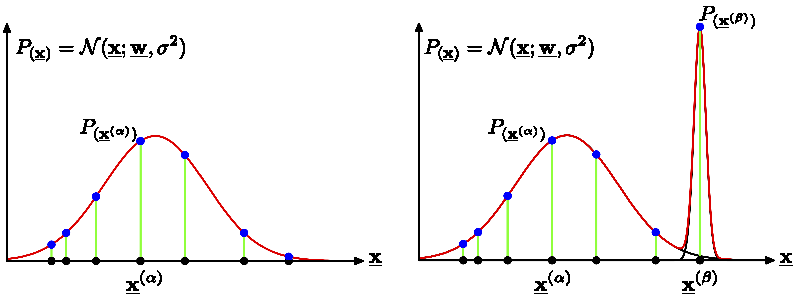
\includegraphics[width=9cm]{section6_fig5}
	\caption{Degenerated solutions}
\end{figure}
\small
\begin{align*}
\mathcal{N}(\vec{x}^{(\beta)}; \vec{w}_{q}, \sigma_q^2) &= \mathcal{N}(\vec{x}^{(\beta)}; \vec{x}^{(\beta)}, \sigma_q^2) 
\\&= \frac{1}{\left( 2\pi \sigma_q^2 \right)^{1/2}} \exp \left\{ - \frac{\left( \vec{x}^{(\beta)} -\vec{x}^{(\beta)} \right)^2}{2 \sigma_q^2} \right\} = \frac{1}{(2\pi)^{1/2}} \frac{1}{\sigma_q} \stackrel{\sigma_q^2 \rightarrow 0}{\longrightarrow} \infty
\end{align*}
$\leadsto$ model validation (testset method) to detect overfitting \\
$\leadsto$ Maximum-a-posteriori instead of maximum likelihood approaches using a prior\\
$\phantom{\leadsto}$ for each component which penalizes components with small variance $\sigma_q^2$
%--------------------------------------------------------------------------------
\paragraph{Hierarchical Gaussian mixtures}\mbox{}\\
\begin{figure}[h]
    \centering
    \begin{subfigure}[b]{0.48\textwidth}
        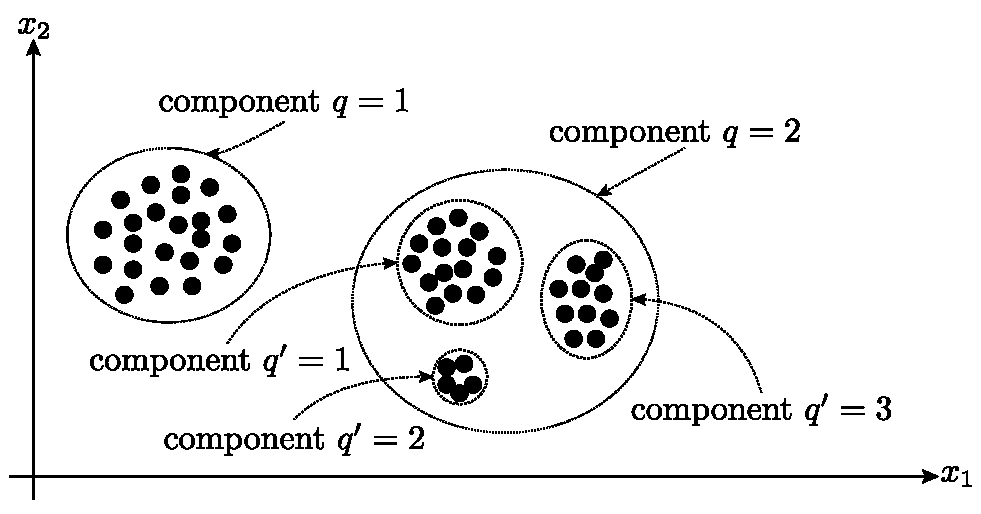
\includegraphics[width=0.9\textwidth]{section6_fig6}
    \end{subfigure}
    \begin{subfigure}[b]{0.48\textwidth}
        \includegraphics[width=0.9\textwidth]{section6_fig7}
    \end{subfigure}
    \caption{Hierarchical Gaussian mixtures}
\end{figure}
\begin{center}
\vspace{0.5cm}
$P_{(\vec{x})} = \sum_{q}^{} P_{(q)} \sum_{q'}^{} P_{(q' | q)} P_{(\vec{x} | q', q)}$
\end{center}
%-------------------------------------------------------------------
\paragraph{Summary}\mbox{}\\
Gaussian mixture model:
\vspace{-0.3cm}
\begin{align*}
P_{(\vec{x})} &= \sum_{q=1}^{M} P_{(q)} P_{(\vec{x} | q)} \\
P_{(\vec{x} | q)} &= \frac{1}{\left( 2\pi \sigma_q^2 \right)^{N/2}} \exp \left\{ - \frac{\left( \vec{x} - \vec{w}_q \right)^2}{2 \sigma_q^2} \right\}
\end{align*}\\
\vspace{0.1cm}
Maximum likelihood:
\vspace{-0.1cm}
\begin{equation*}
P_{(\left\{ \vec{x}^{(\alpha)} \right\} | \text{ parameter})} \eqexcl \max
\end{equation*}\\
\vspace{0.3cm}
Relation to Soft-Clustering:
\vspace{0.1cm}
\begin{itemize}
	\item cost functions are identical, if: $\sigma_q^2 = \text{const.}_{(q)} = \frac{1}{\beta}$ and $P_{(q)} = \text{const.}_{(q)} = \frac{1}{M}$
	\vspace{-0.3cm}
	\item new interpretation of Soft-Clustering:
		\begin{itemize}
			\item estimation of parameter $\vec{w}_q$ of a Gaussian mixture model
			\vspace{0.1cm}
			\item $\beta$ defines the size of the cluster $\widehat{=}$ resolution
		\end{itemize}
\end{itemize}


%--------------------------------------------------------------
\paragraph{Remarks}\mbox{}\\
\begin{itemize}
	\item equivalent solutions (permutation of components)
	\vspace{2mm}
	\item improved initialization by application of the (much faster) $K$-means method: 
	\begin{itemize}
		\item prototypes $\leadsto$ component means $\vec{w}_q$
		\item intra-cluster spreads $\leadsto$ component variances $\sigma_q^2$
	\end{itemize}
	\vspace{2mm}
	\item extension to general Gaussian components ($\sigma_q^2 \rightarrow \vec{\Sigma}_q$) straightforward (cf. Bishop 2006)
	\vspace{2mm}
	\item mixture model: example of latent variable model
\end{itemize}

\subsection{The Expectation-Maximization Algorithm}
\paragraph{Latent variables}\mbox{}\\
Example: mixture model
\begin{itemize}
	\item observed data set $\vec{x}^{(1)}, \dots, \vec{x}^{(p)} \in \mathbb{R}^N$
	\item every data point $\vec{x}^{(\alpha)}$ is generated by one component $q=1, \dots, M$
	\begin{itemize}
		\itl assignment variables: $\vec{m}^{(\alpha)} =  \left( m_1^{(\alpha)}, \dots, m_M^{(\alpha)} \right)^T \in \left\{ 0, 1 \right\}^M$ \\
		\begin{equation*}
		m_q^{(\alpha)} = 
		\begin{cases}
		1, & \text{if component } q \text{ has generated data point} \\
		0, & \text{otherwise}
		\end{cases}
		\hspace{0.5cm}
		 \sum_{q=1}^{M} m_q^{(\alpha)} = 1 
		\end{equation*}
	\end{itemize}
	\item complete data set: $\vec{x}^{(1)}, \vec{m}^{(1)} \dots, \vec{x}^{(p)}, \vec{m}^{(p)}$
	\item hidden / latent variables: $\vec{m}^{(1)}, \dots, \vec{m}^{(p)}$
\end{itemize}


%%%%%%%%%%%%%%%%%%%%%%%%%%%%%%%%%%%%%%%%%%%%%%%%%%%%%%
\paragraph{Latent variable models and maximum likelihood}\mbox{}\\
Calculation of the likelihood of the observed data\\ requires marginalization of $P(\vec{x}, \vec{m} | \vec{w}):$
\begin{equation*}
P \left( \left\{ \vec{x}^{(\alpha)} \right\} | \vec{w} \right) \stackrel{iid}{=} \prod_{\alpha=1}^{p} P \left( \vec{x}^{(\alpha)} | \vec{w} \right) = \prod_{\alpha=1}^{p}  \sum_{\vec{m}} P \left( \vec{x}^{(\alpha)}, \vec{m} | \vec{w} \right)
\end{equation*}
Log-likelihood is computationally costly to maximize / no closed-form solution due to sum in logarithm:

\begin{equation*}
\ln P \left( \left\{ \vec{x}^{(\alpha)} \right\} | \vec{w} \right) = \sum_{\alpha=1}^{p}  \ln \left( \sum_{\vec{m}} P \left( \vec{x}^{(\alpha)}, \vec{m} | \vec{w} \right) \right)
\end{equation*}

%%%%%%%%%%%%%%%%%%%%%%%%%%%%%%%%%%%%%%%%%%%%%%%%%%%%%%
\paragraph{The Expectation-Maximization (EM) algorithm}\mbox{}\\
\small
Maximize the joint distribution over observed and latent variables (specifically useful if $P(\vec{x}, \vec{m} | \vec{w})$ is from the exponential family: Gaussian, Bernoulli etc.) \\
\begin{equation*}
\ln P \left( \left\{ \vec{x}^{(\alpha)} \right\}, \left\{ \vec{m}^{(\alpha)} \right\} \bigg| \vec{w} \right) \eqexcl \max_{(\vec{w})} 
\end{equation*}\\
\vspace{3mm}
Problem: values of the hidden variables are unknown.


%%%%%%%%%%%%%%%%%%%%%%%%%%%%%%%%%%%%%%%%%%%%%%%%%%%%%%
\paragraph{The Expectation-Maximization (EM) algorithm}\mbox{}\\
\scalebox{.9}{   
	\begin{algorithm}[H]
		\DontPrintSemicolon
		choose initial values for the parameters $\vec{w}_\text{old}$ (e.g., by random)	and tolerance $\theta$\;
		\vspace{1mm}
		\Repeat{$| \vec{w}_\text{old} - \vec{w}_\text{new} | < \theta$}{
			\vspace{3mm}
			1. Evaluation of posterior distribution: $P \left( \left\{ \vec{m}^{(\alpha)} \right\} \big| \left\{ \vec{x}^{(\alpha)} \right\} , \vec{w}_{\text{old}} \right)$\;
			\vspace{3mm}
			2. E-Step: Compute expectation of complete data log-likelihood \\
						\hspace{1.5cm} w.r.t posterior of $\left\{ \vec{m}^{(\alpha)} \right\}$
			\vspace{-1mm}
			\begin{equation*}
			\mathcal{Q}(\vec{w}, \vec{w}_{\text{old}}) = \sum_{\left\{ \vec{m}^{(\alpha)} \right\}} P \bigg( \big\{ \vec{m}^{(\alpha)} \big\} \big| \big\{ \vec{x}^{(\alpha)} \big\}, \vec{w}_{\text{old}} \bigg) \ln P \bigg( \big\{ \vec{x}^{(\alpha)} \big\}, \big\{ \vec{m}^{(\alpha)} \big\} \big| \vec{w} \bigg)
			\end{equation*}\;
			\vspace{-5mm}
			3. M-Step: Determine new parameters that maximize the expectation
			\vspace{-1mm}
			\begin{align*}
			\vec{w}_{\text{new}} &= \operatorname{arg} \max_{(\vec{w})} \mathcal{Q}(\vec{w}, \vec{w}_{\text{old}}) \\
			\vec{w}_{\text{old}} &\leftarrow \vec{w}_{\text{new}}
			\end{align*}    
		
		}
	\end{algorithm}
}
%%%%%%%%%%%%%%%%%%%%%%%%%%%%%%%%%%%%%%%%%%%%%%%%%%%%%%
\paragraph{Remarks}\mbox{}\\
\begin{itemize}
	\item The EM algorithm converges to a local maximum of the log-likelihood function (cf. Bishop 2006)
	\item local optima (e.g., multimodal likelihood function) $\leadsto$ different initial conditions or simulated annealing methods
	\item EM is applicable to many latent variable problems: e.g., hidden Markov models, missing data situations
	\item EM is particularly efficient if the complete data distribution is from exponential family (log of exp)
	\item further extensions:
	\begin{itemize}
		\item continuous latent variables (replace sums by integrals in marginalization / expectation)
		\item maximum a posteriori estimation using a prior distribution $P_0(\vec{w})$
		\item non-tractable E- or M-steps: approximate inference or generalized EM-algorithms
	\end{itemize}
\end{itemize}
%%%%%%%%%%%%%%%%%%%%%%%%%%%%%%%%%%%%%%%%%%%%%%%%%%%%%%
\paragraph{Gaussian mixtures revisited}\mbox{}\\
\vspace{-3mm}
\begin{equation*}
P(\vec{x}) = \sum_{q=1}^{M} \rho(q) \mathcal{N}(\vec{x} | \vec{w}_q, \sigma_q^2) \eqexcl \sum_{\vec{m}} P(\vec{x}, \vec{m}) = \sum_{\vec{m}} P(\vec{m}) P(\vec{x} | \vec{m})
\end{equation*}
mixture parameters: $\rho(q)$,\quad $0 \leq \rho(q) \leq 1, \, \sum_{q=1}^{M} \rho(q) = 1$\\
\vspace{2mm}
prior distribution of latent variables 
\vspace{-1mm}
\begin{equation*}
 P(\vec{m}) = \prod_{q=1}^{M} \rho(q)^{m_q}
\end{equation*}
\vspace{2mm}
conditional distribution of the observed variables given the latent variables
\vspace{-1mm}
\begin{equation*}
P(\vec{x} | \vec{m}) = \prod_{q=1}^{M} \mathcal{N}^{m_q}(\vec{x} | \vec{w}_q, \sigma_q^2)
\end{equation*}
joint distribution 
\vspace{-1mm}
\begin{equation*}
P(\vec{x} , \vec{m}) = P(\vec{x} | \vec{m}) \cdot P(\vec{m}) = \prod\limits_{q=1}^{M} \rho(q)^{m_q} \mathcal{N}^{m_q}(\vec{x} | \vec{w}_q, \sigma_q^2)
\end{equation*}


%%%%%%%%%%%%%%%%%%%%%%%%%%%%%%%%%%%%%%%%%%%%%%%%%%%%%%
\paragraph{Gaussian mixtures \& the EM algorithm}\mbox{}\\
joint distribution: $P(\vec{x}, \vec{m}) = \prod\limits_{q=1}^{M} \rho(q)^{m_q} \mathcal{N}^{m_q}(\vec{x} | \vec{w}_q, \sigma_q^2)$ \\
likelihood:
\begin{equation*}
P \left(\left\{ \vec{x}^{(\alpha)} \right\}, \left\{ \vec{m}^{(\alpha)} \right\} \bigg| \left\{ \vec{w}_q, \sigma_q^2, \rho(q) \right\} \right) = \prod_{\alpha=1}^{p} \prod_{q=1}^{M} \rho(q)^{m_q^{(\alpha)}} \mathcal{N}^{m_q^{(\alpha)}}(\vec{x}^{(\alpha)} | \vec{w}_q, \sigma_q^2)
\end{equation*}
log-likelihood:
\begin{equation*}
\ln P \left(\left\{ \vec{x}^{(\alpha)} \right\}, \left\{ \vec{m}^{(\alpha)} \right\} \bigg| \left\{ \vec{w}_q, \sigma_q^2, \rho(q) \right\} \right) = \sum_{\alpha=1}^{p} \sum_{q=1}^{M} m_q^{(\alpha)} \left( \ln \rho(q) + \ln  \mathcal{N}(\vec{x}^{(\alpha)} | \vec{w}_q, \sigma_q^2) \right)
\end{equation*}\\
\vspace{3mm}
log within sum \& log of normal: much easier to handle
posterior distribution: \\
\begin{align*}
P(\vec{m} | \vec{x}) &= \frac{P(\vec{x}, \vec{m})  }{P(\vec{x})} = \frac{\prod_{q=1}^{M} \left[ \rho(q) \mathcal{N}(\vec{x} | \vec{w}_q, \sigma_q^2) \right]^{m_q}}{\sum_{q=1}^{M}  \rho(q) \mathcal{N}(\vec{x} | \vec{w}_q, \sigma_q^2) }
\end{align*}
posterior distribution of hidden data given observed: \\
	\begin{align*}
	P \left( \left\{ \vec{m}^{(\alpha)} \right\} \bigg| \left\{ \vec{x}^{(\alpha)} \right\}, \left\{ \vec{w}_q, \sigma_q^2, \rho(q) \right\} \right) \hspace{4cm}
	\\  \stackrel{\text{iid. data}}{=} \prod_{\alpha=1}^{p} \frac{  P \left( \vec{x}^{(\alpha)} , \vec{m}^{(\alpha)} \big| \left\{ \vec{w}_q, \sigma_q^2, \rho(q) \right\} \right)  }{P \left( \vec{x}^{(\alpha)}  \big| \left\{ \vec{w}_q, \sigma_q^2, \rho(q) \right\} \right)} \hspace{2.5cm}
	\\ = \hspace{3.5mm} \prod_{\alpha=1}^{p} \frac{ \prod_{q=1}^{M} \left[ \rho(q) \mathcal{N}(\vec{x}^{(\alpha)} | \vec{w}_q, \sigma_q^2) \right]^{m_q^{(\alpha)}}  }{ \sum_{q=1}^{M}  \rho(q) \mathcal{N}(\vec{x}^{(\alpha)} | \vec{w}_q, \sigma_q^2)  } \hspace{2.25cm}
	\end{align*}

expected value under posterior: \\
	\begin{align*}
	\langle m_q^{(\alpha)} \rangle_{ P \left( \left\{ \vec{m}^{(\alpha)} \right\} \big| \left\{ \vec{x}^{(\alpha)} \right\}, \left\{ \vec{w}_q, \sigma_q^2, \rho(q) \right\} \right) } &= \textbf{ see blackboard}
	\\&= \frac{\rho(q) \mathcal{N}(\vec{x}^{(\alpha)} | \vec{w}_q, \sigma_q^2)}{\sum\limits_{r=1}^{M}  \rho(r) \mathcal{N}(\vec{x}^{(\alpha)}  | \vec{w}_r, \sigma_r^2)} 
	\\ &= \rho(q | \vec{x}^{(\alpha)}) \text{ (\small{from mixture EM-Algorithm) }}
	\end{align*}
	
	\newcommand{\OLD}{\textnormal{\tiny \textsc{old}}}
	using this we can evaluate\\
	\vspace{-0.4cm}
	\begin{align*}
	\mathcal{Q}  &\left(  \left\{ \vec{w}_q, \sigma_q^2, \rho(q) \right\}, \left\{ \vec{w}_q, \sigma_q^2, \rho(q) \right\}_{\OLD} \right) 
	\\&= \bigg\langle \ln P \left( \left\{ \vec{x}^{(\alpha)} \right\}, \left\{ \vec{m}^{(\alpha)} \right\} \bigg| \left\{ \vec{w}_q, \sigma_q^2, \rho(q) \right\} \right) \bigg\rangle_{ P \left( \left\{ \vec{m}^{(\alpha)} \right\} \big| \left\{ \vec{x}^{(\alpha)} \right\}, \left\{ \vec{w}_q, \sigma_q^2, \rho(q) \right\}_\OLD \right) }
	\\ &= \bigg\langle \sum_{\alpha=1}^{p} \sum_{q=1}^{M} m_q^{(\alpha)} \left(  \ln \rho(q) + \ln \mathcal{N}\left( \vec{x}^{(\alpha)} \big| \vec{w}_q, \sigma_q^2 \right) \right) \bigg\rangle_{ P \left( \left\{ \vec{m}^{(\alpha)} \right\} \big| \left\{ \vec{x}^{(\alpha)} \right\}, \left\{ \vec{w}_q, \sigma_q^2, \rho(q) \right\}_\OLD \right) }
	\\& = \sum_{\alpha=1}^{p} \sum_{q=1}^{M} \left[ \langle m_q^{(\alpha)} \rangle_{ P \left( \left\{ \vec{m}^{(\alpha)} \right\} \big| \left\{ \vec{x}^{(\alpha)} \right\}, \left\{ \vec{w}_q, \sigma_q^2, \rho(q) \right\}_\OLD \right) } \cdot \left(  \ln \rho(q) + \ln \mathcal{N}\left( \vec{x}^{(\alpha)} \big| \vec{w}_q, \sigma_q^2 \right) \right) \right]
	\\& = \sum_{\alpha=1}^{p} \sum_{q=1}^{M} \left[ \rho \left( q | \vec{x}^{(\alpha)} \right) \cdot \left(  \ln \rho(q) + \ln \mathcal{N}\left( \vec{x}^{(\alpha)} \big| \vec{w}_q, \sigma_q^2 \right) \right)  \right]
	\end{align*}\\
	\vspace{1mm}
	$\leadsto$ E-step: calculation of 
	\begin{equation*}
	\rho \left( q | \vec{x}^{(\alpha)} \right) = \frac{ \rho(q)_\OLD \cdot \mathcal{N} \left(\vec{x}^{(\alpha)} | \vec{w}_{q, \OLD}  , \sigma_{q,\OLD}^2  \right) }{  \sum_{r=1}^{M} \rho(r)_\OLD \cdot \mathcal{N} \left(\vec{x}^{(\alpha)} | \vec{w}_{r,\OLD}  , \sigma_{r,\OLD}^2  \right) }
	\end{equation*}
	
	
calculation of new parameters:\\
 $\left\{ \vec{w}_q, \sigma_q^2, \rho(q) \right\}_{\text{new}} = \argmax\limits_{\left\{ \vec{w}_q, \sigma_q^2, \rho(q) \right\}} \mathcal{Q}  \left(  \left\{ \vec{w}_q, \sigma_q^2, \rho(q) \right\}, \left\{ \vec{w}_q, \sigma_q^2, \rho(q) \right\}_{\OLD} \right)$\\
\begin{align*}
\mathcal{Q}  &\left(  \left\{ \vec{w}_q, \sigma_q^2, \rho(q) \right\}, \left\{ \vec{w}_q, \sigma_q^2, \rho(q) \right\}_{\OLD} \right) 
\\&= \sum_{\alpha=1}^{p} \sum_{q=1}^{M} \left[ \rho \left( q | \vec{x}^{(\alpha)} \right) \cdot \left(  \ln \rho(q) + \ln \mathcal{N}\left( \vec{x}^{(\alpha)} \big| \vec{w}_q, \sigma_q^2 \right) \right)  \right]
\end{align*}
\newpage
\begin{table}
	\begin{tabular}{rlc}
		$\frac{\partial \mathcal{Q}}{\partial \vec{w}_q} = 0 \quad \Rightarrow$ & $\hspace{1mm} \vec{w}_{q,\text{new}} = \frac{\sum_{\alpha=1}^{p} \rho(q | \vec{x}^{(\alpha)}) \vec{x}^{(\alpha)} }{\sum_{\alpha=1}^{p} \rho(q | \vec{x}^{(\alpha)}) }$ & \rdelim\}{6}{100pt}[$\substack{\text{ expressions from}\\\text{mixture EM-algorithm}\\ \text{recovered}}$ ]  \\[10pt]               
		$\frac{\partial \mathcal{Q}}{\partial \sigma_q^2} = 0 \quad \Rightarrow$ & $\hspace{0.2cm} \sigma_{q,\text{new}}^2 = \frac{1}{N} \frac{\sum_{\alpha=1}^{p} \left( \vec{x}^{(\alpha)} -  \vec{w}_{q,\OLD} \right)^2 \rho(q | \vec{x}^{(\alpha)} )  }{ \sum_{\alpha=1}^{p}  \rho(q | \vec{x}^{(\alpha)}} $ &                         \\[14pt]              
		$\frac{\partial \mathcal{Q}}{\partial \rho(q)} = 0 \quad \Rightarrow$ & $\rho(q)_{\text{new}} = \frac{1}{p} \sum_{\alpha=1}^{p} \rho(q | \vec{x}^{(\alpha)})$ &                         \\[5pt]                
	\end{tabular}
\end{table}
$\leadsto$ M-step: optimal parameters for given 
\begin{equation*}
\langle m_q^{(\alpha)} \rangle_{ P \left( \left\{ \vec{m}^{(\alpha)} \right\} \big| \left\{ \vec{x}^{(\alpha)} \right\}, \left\{ \vec{w}_q, \sigma_q^2, \rho(q) \right\}_\OLD \right) } = \rho \left( q | \vec{x}^{(\alpha)} \right)
\end{equation*}
 